% Options for packages loaded elsewhere
\PassOptionsToPackage{unicode}{hyperref}
\PassOptionsToPackage{hyphens}{url}
%
\documentclass[
]{article}
\usepackage{amsmath,amssymb}
\usepackage{lmodern}
\usepackage{iftex}
\ifPDFTeX
  \usepackage[T1]{fontenc}
  \usepackage[utf8]{inputenc}
  \usepackage{textcomp} % provide euro and other symbols
\else % if luatex or xetex
  \usepackage{unicode-math}
  \defaultfontfeatures{Scale=MatchLowercase}
  \defaultfontfeatures[\rmfamily]{Ligatures=TeX,Scale=1}
\fi
% Use upquote if available, for straight quotes in verbatim environments
\IfFileExists{upquote.sty}{\usepackage{upquote}}{}
\IfFileExists{microtype.sty}{% use microtype if available
  \usepackage[]{microtype}
  \UseMicrotypeSet[protrusion]{basicmath} % disable protrusion for tt fonts
}{}
\makeatletter
\@ifundefined{KOMAClassName}{% if non-KOMA class
  \IfFileExists{parskip.sty}{%
    \usepackage{parskip}
  }{% else
    \setlength{\parindent}{0pt}
    \setlength{\parskip}{6pt plus 2pt minus 1pt}}
}{% if KOMA class
  \KOMAoptions{parskip=half}}
\makeatother
\usepackage{xcolor}
\usepackage{graphicx}
\makeatletter
\def\maxwidth{\ifdim\Gin@nat@width>\linewidth\linewidth\else\Gin@nat@width\fi}
\def\maxheight{\ifdim\Gin@nat@height>\textheight\textheight\else\Gin@nat@height\fi}
\makeatother
% Scale images if necessary, so that they will not overflow the page
% margins by default, and it is still possible to overwrite the defaults
% using explicit options in \includegraphics[width, height, ...]{}
\setkeys{Gin}{width=\maxwidth,height=\maxheight,keepaspectratio}
% Set default figure placement to htbp
\makeatletter
\def\fps@figure{htbp}
\makeatother
\usepackage[normalem]{ulem}
\setlength{\emergencystretch}{3em} % prevent overfull lines
\providecommand{\tightlist}{%
  \setlength{\itemsep}{0pt}\setlength{\parskip}{0pt}}
\setcounter{secnumdepth}{-\maxdimen} % remove section numbering
\ifLuaTeX
  \usepackage{selnolig}  % disable illegal ligatures
\fi
\IfFileExists{bookmark.sty}{\usepackage{bookmark}}{\usepackage{hyperref}}
\IfFileExists{xurl.sty}{\usepackage{xurl}}{} % add URL line breaks if available
\urlstyle{same} % disable monospaced font for URLs
\hypersetup{
  hidelinks,
  pdfcreator={LaTeX via pandoc}}

\author{}
\date{}

\begin{document}

\hypertarget{cse-5370-bio-informatics}{%
\section{\texorpdfstring{\textbf{\uline{CSE 5370:
BIO-INFORMATICS}}}{CSE 5370: BIO-INFORMATICS}}\label{cse-5370-bio-informatics}}

\hypertarget{homework-3}{%
\section{\texorpdfstring{\textbf{\uline{HOMEWORK --
3}}}{HOMEWORK -- 3}}\label{homework-3}}

\hypertarget{section}{%
\section{}\label{section}}

\hypertarget{substution-matrices}{%
\subsection{\texorpdfstring{\textbf{Substution
Matrices}}{Substution Matrices}}\label{substution-matrices}}

The transition mutations (A ←→ G and T ←→ C) are less common than
transversions (A ←→ T , A ←→ C, G ←→ T , and G ←→ C).To create a
substitution matrix that reflects the lower frequency of transition
mutations, we can use the following values:

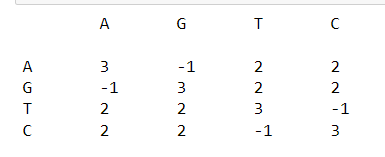
\includegraphics[width=3.20861in,height=1.30845in]{1.png}

Here, the transition mutations have a penalty of -1, while the
transversion mutations have a penalty of 2 and match score is 3. This
results in a higher penalty for transversions, reflecting their lower
frequency.

\hypertarget{global-alignment}{%
\subsection{\texorpdfstring{\textbf{Global
Alignment}}{Global Alignment}}\label{global-alignment}}

Implemented the Needleman-Wunsch algorithm and returned the possible
alignments, and also took multiple examples that we discussed in class
to crosscheck the correctness.

\hypertarget{local-alignment}{%
\subsection{\texorpdfstring{\textbf{Local
Alignment}}{Local Alignment}}\label{local-alignment}}

Implemented the Smith-Waterman algorithm and returned the possible
alignments, and also took multiple examples that we discussed in class
to crosscheck the correctness.

And as discussed in class, it is printing the output as expected and
used pretty print.

\hypertarget{section-1}{%
\subsection{}\label{section-1}}

\hypertarget{custom-alignment}{%
\subsection{\texorpdfstring{\textbf{Custom
Alignment}}{Custom Alignment}}\label{custom-alignment}}

Written code to create substation matrix that will store in
1002059166\_S.txt, and used that substation matrix, local alignment to
print the possible alignments and matrix in 1002059166\_D.txt.

Here is the below possible Alignments for my name sravanchandaka and
given string.

{[}(\textquotesingle ch\textquotesingle,
\textquotesingle ck\textquotesingle){]}

{[}(\textquotesingle vanch\textquotesingle,
\textquotesingle verth\textquotesingle){]}

{[}(\textquotesingle chan\textquotesingle,
\textquotesingle ckbr\textquotesingle){]}

{[}(\textquotesingle ak\textquotesingle,
\textquotesingle ck\textquotesingle){]}

\hypertarget{section-2}{%
\subsection{}\label{section-2}}

\hypertarget{section-3}{%
\subsection{}\label{section-3}}

\hypertarget{difficulty-adjustment}{%
\subsection{\texorpdfstring{\textbf{5) Difficulty
Adjustment}}{5) Difficulty Adjustment}}\label{difficulty-adjustment}}

In total assignment took more than 23 hours to complete, initially to
understand the concept took some time.

The implementation of Custom Alignment and understanding the concept is
difficult, as multiple arrows need to be printed in the matrix it is
challenging.

\end{document}
